\section{Methods}


\subsection{Project Methodology}
When working in a project it is generally a good idea to work according to a predetermined project methodology model. This tends to make the work more effective and produce better quality. That is, more is produced during the same amount of time, the final product is more thought out, better teamwork etc.

Simply, if you have a plan at the start it is easier to stick to that plan and stay on the same path as intended, rather than shifting to another one. That is not to say that the plan cannot change, but if it does it does so controllably.

A historically good model has been the waterfall model. However, in the software industry this has changed lately with the agile methodology being more popular and has proven to be very effective.

\subsubsection{Agile}
Basically, the agile model says that rather than planning a workload for 6 months forward or so it is better to work in short iterations.

-- More on how the agile model works --

For our planned work we have decided to work in two week period sprints where we begin on a Tuesday and end on a Monday. At each start of a sprint we pick out stories to focus on for the coming two weeks and try to estimate how long each of them will take.
On weekdays we start with a quick discussion about yesterdays work and what we are planning to do today. This is for everyone to be up to speed about the other persons work.
At the end of the sprint everything is review and analysed so to do even better the next sprint by correcting possible faults.

-- Text and picture explaining our board --




\subsection{Matlab prototype}


\subsection{Tensorflow and Machine Learning}

\subsection{AR implementation in ARKit}

\begin{figure}[hbtp]
\begin{center}
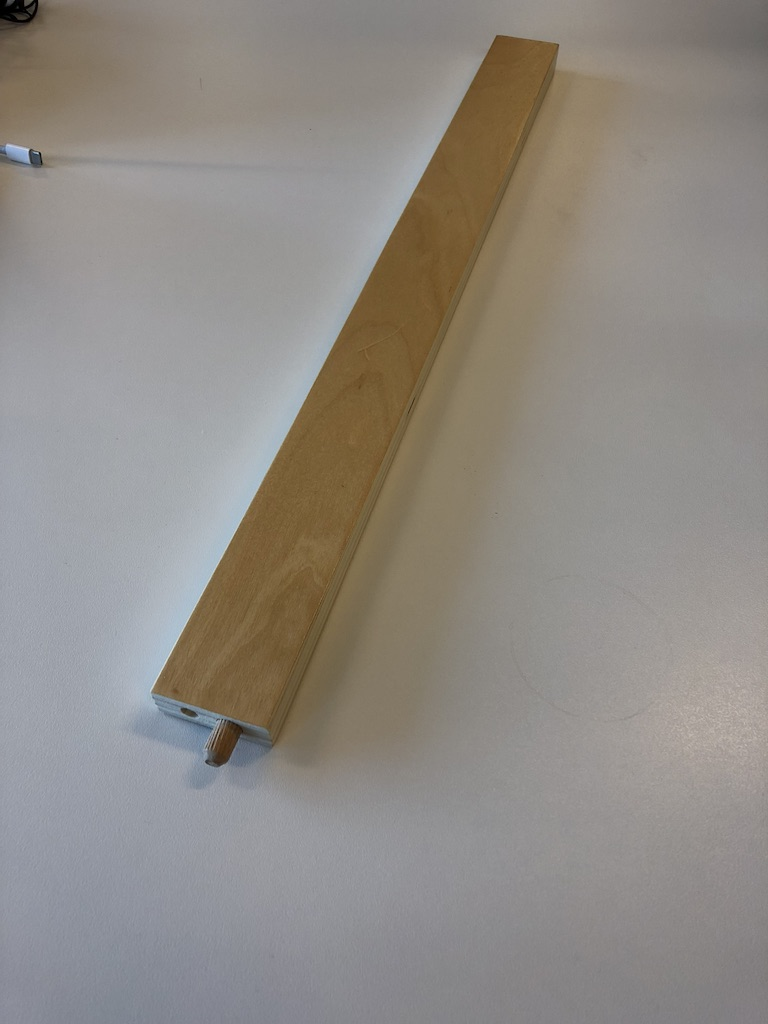
\includegraphics[width = 0.5\textwidth]{./Images/im1.jpg} 
\caption{Example image}
\end{center}
\end{figure}

\newpage

\begin{center}
\textbf{Log book}
\end{center}

\textbf{2018-09-18}
When training the object recognition net, they where trained on only the red channel and although it technically worked by inputting an RGB image later on, it obviously gave us completely bogus results.